\section{Key Concepts for Adaptive Reading Analytics}
\label{sec:key-concepts}
This section defines the core concepts underlying the thesis.
Definitions are grounded in primary and project-aligned sources.

\subsection{Adaptive Reading System}
\label{subsec:adaptive-reading-system}
The "Reading the Reader" concept assumes a closed-loop system that senses gaze-related signals (including pupil size) during reading, extracts higher-level events (fixations, saccades, regressions), classifies reading state or style, and triggers typographic interventions in real time \cite{dtucompute2025rtr}.
Fig.~\ref{fig:adaptive-loop} depicts this loop as four sequential stages, sensing, analysis, decision, and intervention, whose output changes what the reader sees and so feeds the next cycle of sensing.
Treating each stage as an independently replaceable module behind a stable contract is the central architectural commitment of this thesis, and it is the property examined in the chapters that follow.

\usetikzlibrary{arrows.meta, positioning, fit, backgrounds}
\begin{figure}[htbp]
\centering
\resizebox{0.98\linewidth}{!}{%
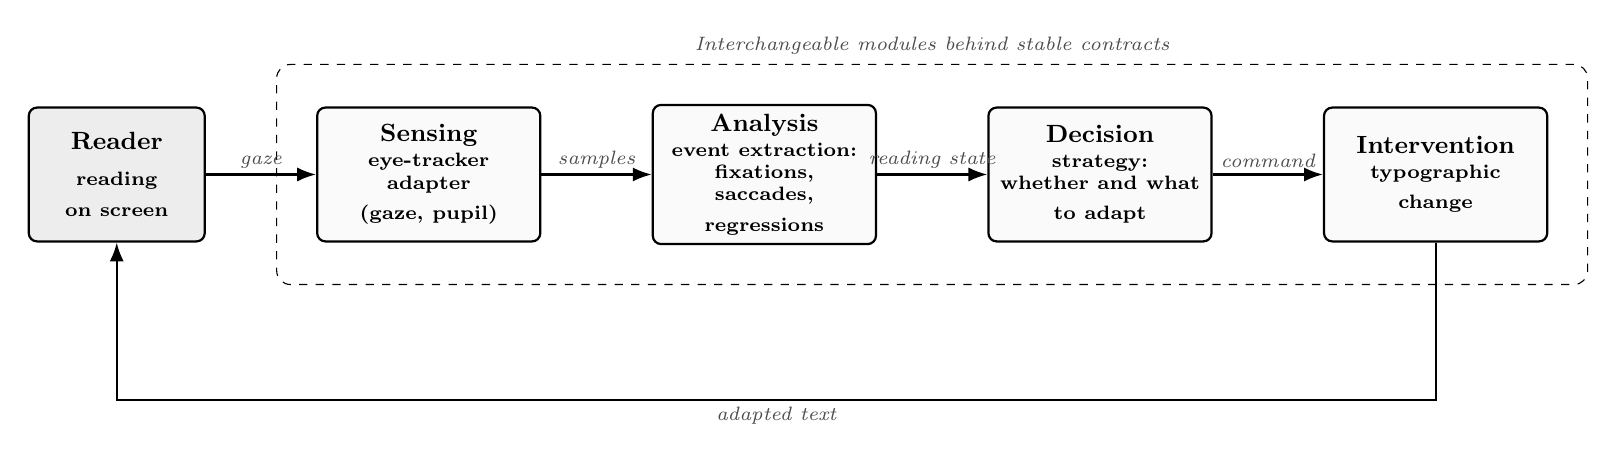
\begin{tikzpicture}[
  mod/.style={draw, thick, rounded corners=3pt, align=center,
              text width=2.6cm, minimum height=1.7cm, font=\small, fill=gray!4},
  reader/.style={draw, thick, rounded corners=3pt, align=center,
                 text width=2.0cm, minimum height=1.7cm, font=\small, fill=gray!14},
  flow/.style={-{Latex[length=2.4mm]}, thick},
  io/.style={font=\scriptsize\itshape, text=black!70, inner sep=2pt},
  node distance=14mm
]

\node[reader] (reader) {\bfseries Reader\\[2pt]\scriptsize reading on screen};
\node[mod, right=of reader] (sense)   {\bfseries Sensing\\[1pt]\scriptsize eye-tracker adapter\\\scriptsize (gaze, pupil)};
\node[mod, right=of sense]   (analyse) {\bfseries Analysis\\[1pt]\scriptsize event extraction:\\\scriptsize fixations, saccades,\\\scriptsize regressions};
\node[mod, right=of analyse] (decide)  {\bfseries Decision\\[1pt]\scriptsize strategy:\\\scriptsize whether and what\\\scriptsize to adapt};
\node[mod, right=of decide]  (act)     {\bfseries Intervention\\[1pt]\scriptsize typographic\\\scriptsize change};

\draw[flow] (reader)  -- node[io, above]{gaze}          (sense);
\draw[flow] (sense)   -- node[io, above]{samples}       (analyse);
\draw[flow] (analyse) -- node[io, above]{reading state} (decide);
\draw[flow] (decide)  -- node[io, above]{command}       (act);

\draw[flow] (act.south) -- ++(0,-2.0) -| node[io, below, pos=0.25]{adapted text} (reader.south);

\begin{scope}[on background layer]
\node[draw, dashed, rounded corners=5pt, fit=(sense)(analyse)(decide)(act),
      inner sep=5mm,
      label={[font=\scriptsize\itshape, text=black!70]above:Interchangeable modules behind stable contracts}] {};
\end{scope}

\end{tikzpicture}%
}
\caption{The closed-loop adaptive reading concept. Gaze and pupil signals from the reader are sensed, reduced to oculomotor events, classified into a reading state, and used to decide and apply a typographic intervention, which changes what the reader sees and thereby closes the loop. The four stages are designed as interchangeable modules behind stable contracts.}
\label{fig:adaptive-loop}
\end{figure}

\subsection{Micro-Interventions and Just-in-Time Adaptation}
\label{subsec:micro-interventions}
Micro-interventions are an established pattern in digital-health software rather than a term coined here.
Persson et al. synthesise this literature into the Design for Microintervention Software Technology (D-MIST) framework, which organises a micro-intervention system into three levels: the narrative, or the consolidated experience of engaging with many micro-interventions toward an overarching goal; the micro-intervention itself, a focused intervention composed of self-contained events; and the event, a single momentary change delivered through a resource \cite{persson2025microintervention}.
The Reading the Reader proposal adapts this concept to reading, framing micro-interventions as small, context-preserving changes to typography or layout (for example, spacing or contrast adjustments) that support reading without disrupting flow \cite{dtucompute2025rtr}.

In this thesis, just-in-time adaptation is the term we use for an intervention policy that fires on short temporal windows of online gaze and interaction features rather than on a fixed schedule.
We define it operationally as a policy that triggers within such a window while controlling for two quantities: the intervention cost, meaning the risk of disrupting reading, and the recovery behaviour, meaning the time the reader needs to resume reading afterwards.

\subsection{Context Preservation and Recovery Metrics}
\label{subsec:context-preservation}
Recent work presented at the Symposium on Eye Tracking Research and Applications (ETRA) frames context preservation as interface functionality that enables readers to resume reading quickly after a typographic change.
It introduces the metric Reading Resume Time (RRT) and compares four intervention designs (Popup, Undo, Notification, and Gradual) on the time a reader takes to recover after the change \cite{jensen2025context}.

Jensen et al. report that, among the four designs, only the gradual intervention combined with highlighting produced a statistically significant reduction in intervention time, falling from 14.9~s without highlighting to 4.0~s with it (Mann-Whitney U, p < .001), while the gradual design was also associated with the lowest reported recovery difficulty \cite{jensen2025context}.
This indicates that intervention form factor and transition smoothness materially affect how quickly reading recovers.

This thesis treats context preservation as a first-class design goal whose effect should be observable rather than assumed.
We therefore propose to instrument the runtime so that candidate recovery measures, such as Reading Resume Time, the time taken for gaze to restabilise after a change, and any burst of regressions that follows it, can be logged and compared in future studies, rather than claiming a measured recovery result for any single intervention in this work.

\subsection{Central Vision Loss and Reading}
\label{subsec:central-vision-loss}
The Reading the Reader project targets readers whose central vision is impaired, most commonly through age-related macular degeneration (AMD).
Central vision loss (CVL) damages the part of the visual field used for high-acuity tasks, forcing affected readers to rely on peripheral or parafoveal vision and producing measurable declines in reading speed and changes in eye-movement patterns \cite{kanonidou2011reading}.
Reading is therefore not a single perceptual act but a combination of sensory, motor, and cognitive processes that CVL disrupts simultaneously.

Interventions that adapt presentation to the individual reader have been studied as a way to recover some of this lost performance.
Perceptual-learning regimes have been reported to improve reading speed in people with long-standing central vision loss \cite{chung2011improving},
and a broader literature surveys clinical and technological strategies for training reading skills in central-field-loss patients \cite{cocomartin2020training}.
Mobile and digital assistive technologies have been positioned as a discreet, widely available route to supporting visually impaired readers in everyday settings \cite{hakobyan2013mobile}.
A distinction of scope is important here.
Central vision loss is the motivating target condition for the wider Reading the Reader project, but the reading sessions in this thesis are conducted with general laboratory participants rather than recruited CVL patients.
The platform is therefore designed to serve CVL readers eventually, while the present work validates the architecture and runtime rather than a clinical outcome.
This thesis does not pursue a clinical training protocol; it treats CVL as the condition that justifies real-time, individualised typographic adaptation and that frames why minimising disruption (Sec.~\ref{subsec:context-preservation}) matters.

\subsection{Oculomotor Events: Fixations, Saccades, and Regressions}
\label{subsec:oculomotor-events}
Gaze during reading is not continuous but decomposes into discrete oculomotor events.
A fixation is a relatively stable gaze on a small region, during which visual information is extracted; a saccade is the rapid ballistic movement that relocates the gaze between fixations \cite{salvucci2000identifying}.
A regression is a backward saccade against the reading direction and is commonly associated with processing or comprehension difficulty \cite{guan2022predictive}.
Fig.~\ref{fig:oculomotor} illustrates a representative scan path over one line of text, with fixations coloured by the order in which they occur, the forward saccades that connect them, and a single regression back to an earlier word.

\usetikzlibrary{arrows.meta}
\definecolor{fixearly}{HTML}{157F3B}
\definecolor{fixlate}{HTML}{EFE32B}
\definecolor{saccol}{HTML}{555555}
\definecolor{regcol}{HTML}{C0392B}
\begin{figure}[htbp]
\centering
\resizebox{0.92\linewidth}{!}{%
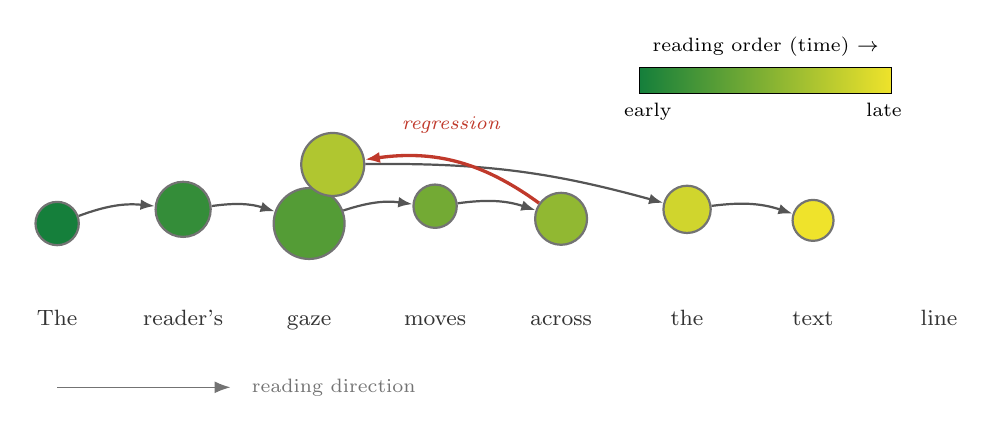
\begin{tikzpicture}[
  fix/.style={circle, draw=black!55, thick, inner sep=0pt},
  word/.style={font=\footnotesize, text=black!80, anchor=base},
  sacc/.style={-{Latex[length=1.8mm]}, thick, saccol},
  regr/.style={-{Latex[length=1.9mm]}, very thick, regcol},
  ann/.style={font=\scriptsize\itshape}
]

% Words (a single line of text)
\node[word] (t1) at (0,0)    {The};
\node[word] (t2) at (1.6,0)  {reader's};
\node[word] (t3) at (3.2,0)  {gaze};
\node[word] (t4) at (4.8,0)  {moves};
\node[word] (t5) at (6.4,0)  {across};
\node[word] (t6) at (8.0,0)  {the};
\node[word] (t7) at (9.6,0)  {text};
\node[word] (t8) at (11.2,0) {line};

% Fixations in temporal order (fill = reading order/time; size = dwell duration).
% f6 is a regressive re-fixation of "gaze", raised slightly to stay visible.
\node[fix, minimum size=0.55cm, fill=fixearly]            (f1) at (0,1.30)   {};
\node[fix, minimum size=0.70cm, fill=fixlate!14!fixearly] (f2) at (1.6,1.48) {};
\node[fix, minimum size=0.90cm, fill=fixlate!29!fixearly] (f3) at (3.2,1.30) {};
\node[fix, minimum size=0.55cm, fill=fixlate!43!fixearly] (f4) at (4.8,1.52) {};
\node[fix, minimum size=0.66cm, fill=fixlate!57!fixearly] (f5) at (6.4,1.36) {};
\node[fix, minimum size=0.80cm, fill=fixlate!71!fixearly] (f6) at (3.5,2.05) {};
\node[fix, minimum size=0.60cm, fill=fixlate!86!fixearly] (f7) at (8.0,1.48) {};
\node[fix, minimum size=0.52cm, fill=fixlate]             (f8) at (9.6,1.34) {};

% Forward saccades (temporal order)
\draw[sacc] (f1) to[bend left=13] (f2);
\draw[sacc] (f2) to[bend left=13] (f3);
\draw[sacc] (f3) to[bend left=13] (f4);
\draw[sacc] (f4) to[bend left=13] (f5);
\draw[sacc] (f6) to[bend left=8]  (f7);
\draw[sacc] (f7) to[bend left=13] (f8);

% Regression (backward saccade against reading direction)
\draw[regr] (f5) to[bend right=22] (f6);
\node[ann, regcol] at (5.0,2.55) {regression};

% Time legend (gradient bar)
\shade[left color=fixearly, right color=fixlate] (7.4,2.95) rectangle (10.6,3.28);
\draw (7.4,2.95) rectangle (10.6,3.28);
\node[font=\scriptsize, anchor=south] at (9.0,3.30) {reading order (time) $\rightarrow$};
\node[font=\scriptsize, anchor=north] at (7.5,2.95) {early};
\node[font=\scriptsize, anchor=north] at (10.5,2.95) {late};

% Reading-direction hint
\draw[-{Latex[length=2mm]}, black!55] (0,-0.78) -- (2.2,-0.78);
\node[font=\scriptsize, text=black!55, anchor=west] at (2.35,-0.78) {reading direction};

\end{tikzpicture}%
}
\caption{A representative scan path over a single line of text, encoding the temporal dimension of reading. Each circle is a fixation, positioned over the word it lands on, with circle area indicating dwell duration and fill colour indicating the order in which fixations occur (legend). Grey arrows are forward saccades that advance along the line; the red arrow is a regression, a backward saccade that re-fixates an earlier word (here "gaze") and is commonly associated with processing difficulty.}
\label{fig:oculomotor}
\end{figure}

Extracting these events from a raw gaze stream is the task of fixation-identification algorithms, for which Salvucci and Goldberg proposed an influential taxonomy organised by the criterion each algorithm uses, such as velocity, dispersion, or area of interest \cite{salvucci2000identifying}.
The platform developed in this thesis performs this extraction online using the area-of-interest variant of that taxonomy: each gaze observation is first resolved to the word it falls on, and the dwell time on that word is thresholded into fixations and saccades, so that downstream decision strategies can reason over reading behaviour rather than over raw coordinates.
These definitions therefore underpin the sensing and analysis layers described in later chapters.

\subsection{Typography as an Intervention Medium}
\label{subsec:typography-medium}
The adaptations this thesis applies are typographic: changes to font, size, weight, spacing, and contrast.
This choice is grounded in evidence that such variables measurably affect readability.
Adjustable typography has been argued as a route to low-vision text accessibility \cite{arditi2004adjustable}, and controlled studies report that increased letter spacing and greater letter width improve reading acuity for low-vision readers \cite{beier2021letterspacing}, that font size and line spacing affect online readability \cite{rello2016makeitbig}, and that background colour influences reading performance \cite{rello2017backgroundcolors}.
Eye-tracking has itself been used to study how font size and type influence online reading \cite{beymer2008eyetracking}.

Taken together, these findings define the parameter space within which micro-interventions (Sec.~\ref{subsec:micro-interventions}) operate.
They justify treating typography as the actuator of the adaptive loop while leaving the decision of which adjustment to make, and when, to the interchangeable strategy modules that are the architectural focus of this thesis.
